\documentclass[10pt, a4paper]{article}

\usepackage[a4paper, top=0.5cm, bottom=0.5cm, left=0.5cm, right=0.5cm, landscape]{geometry}
\usepackage{mathtools}
\usepackage{amsfonts}
\usepackage{multicol}
\usepackage{setspace}
\usepackage{graphicx}
\usepackage[dvipsnames]{xcolor}
\usepackage{array}



\author{Zachary Chua Yan Ern}
\date{April 2022}
\setstretch{1.25}

\newcommand{\highlight}[1]{{\color{red}\textbf{#1}}}
\newcommand{\blue}[1]{{\color{MidnightBlue}#1}}
\newcommand{\red}[1]{{\color{red}#1}}
\newcommand{\green}[1]{{\color{ForestGreen}#1}}
\newcommand{\header}[1]{{\normalsize\textbf{#1}}}
\newcommand{\tab}[0]{\hspace*{2mm}}

\begin{document}
	\scriptsize %small
	\setlength\parindent{0pt}
	\setlength{\columnseprule}{0.1pt}
	
	\begin{center}
		{\large ST2131 CheatSheet}\\
		by Zachary Chua
	\end{center}

	\begin{multicols*}{3}
		\header{Counting}

		\textbf{Sample Space}: Set of all possible outcomes of an experiment

		\textbf{Event}: Subset of sample space

		\textbf{Naive definition of probability}: Assumes all outcomes are \blue{equally likely}

		$P(A) = \frac{|A|}{|S|}$, where A is an event

		\red{Limitations} --- not equally likely, infinitely many outcomes

		\red{Note}: if numerator ordered, then denom also ordered and vice versa

		\textbf{Product Rule}: compound experiment with sub-experiments A and B, A has $a$ possible outcomes
		B has $b$ possible outcomes, compound experiment has $ab$ possible outcomes

		\textbf{Binomial Coefficient}: $nCk = \frac{n!}{(n - k)!k!}, 0 \leq k \leq n$

		\textbf{Sampling}

		1. \textbf{Order matters, w replacement}: $n^k$

		2. \textbf{Order matters, w/o replacement}: $n(n-1)\dots(n-k+1)$

		3. \textbf{Order \red{doesn't} matter, w replacment}: $\binom{n + k - 1}{k}$

		\tab{} - Stars and Bars, n boxes, k \underline{indistinguishable} balls

		\tab{} - no. of nonneg integer solns to $x_1 + x_2 + \dots + x_n = k$

		4. \textbf{Order \red{doesn't} matter, w/o replacement}: $\binom{n}{k}$

		\textbf{Vandermonde's Identity}: $\binom{m + n}{k} = \sum_{j =0}^{k} \binom{m}{j} \binom{n}{k - j}$

		\tab{} - m parrots, n eagles, select k birds and select j parrots, select k - j eagles

		\textbf{Axioms of Probability}

		1. $P(\null) = 0, P(S) = 1$

		2. $P(\bigcup_{n = 1}^{\infty} A_n) = \sum_{n = 1}^{\infty} P(A_n)$ if $A_n$ are disjoint events
		
		\tab{} - Disjoint = mutually exclusive and non-overlapping

		\textbf{Inclusion-Exclusion}: prob of union

		$P(\bigcup_{i = 1}^{n} A_i) = \sum_{i} P(A_i) - \sum_{i < j} P(A_i \cap A_j) + \dots + (-1)^{n + 1}P(A_1 \cap \dots \cap A_n)$
	
		Try to look for symmetry to remove terms, or intersections = 0, then higher intersections = 0 also

		\textbf{Probability of intersection}

		$P(A_1 \cap \dots \cap A_n) = P(A_1)P(A_2 | A_1)P(A_3|A_1, A_2)\dots P(A_n | A_1, \dots , A_{n - 1})$

		\textbf{Bayes}: $P(A | B) = \frac{P(B|A)(A)}{P(B)}$

		\red{Note}: $P(A|B) \neq P(B|A)$, Prosecutor's fallacy

		\textbf{Law of Total Probability (LOTP)}: $P(B) = \sum_{j = 1}^{n} P(B|A_j)P(A_j)$

		if $A_1 \dots A_n$ is a \underline{partition} of S

		\textbf{Conditional Independence}: $P(A, B|C) = P(A|C)P(B|C)$

		\red{Note}: Indep $ \not\rightarrow$ Cond Indep and vice versa

		\textbf{Difference Equation}: $X_n = a X_{n-1} b X_{n-2}$

		Guess $X_n = \alpha^n, \alpha \neq 0$

		then $\alpha^2 - \alpha a - b = 0$, let $\alpha_1, \alpha_2$ be the roots

		then $\alpha_1^n, \alpha_2^n$, general solution is $c_1 \alpha_1^n + c_2 \alpha_2^n$\\

		\header{Discrete Distributions}
		
		\textbf{Random Variable}: function that maps for sample space to real line

		Every R.V. has a distribution, whic specifies all probabilities for that r.v

		\red{Note}: PMF $\geq 0$, sums to 1

		\textbf{Expectation:} $E(X) = \sum_{x} xP(X=x)$

		1. $E(cX) = cE(X)$

		2. $E(X + Y) = E(X) + E(Y)$

		\textbf{Indicator RV}: I(A) = 1 if A, 0 otherwise, $E(I(A)) = P(A)$

		\textbf{LOTUS}: $Y = g(X), E(Y) = \sum_{x} g(x) P(X = x)$

		\textbf{Variance}: Distance of r.v from its mean

		1. $Var(X) = E((X - \mu)^2) = E(X^2) - EX^2$

		2. $Var(X) \geq 0$, if equal to 0, then r.v is constant 

		3. $Var(cX) = c^2Var(X)$

		4. $Var(X + Y) \neq Var(X) + Var(Y)$, unless X and Y are \underline{independent}

		5. $Var(X + c) = Var(X)$

		\textbf{Bernoulli}: $X \sim Bern(p)$
		
		PMF: $P(X = 1) = p, P(X = 0) = 1-p, 0 \leq p \leq 1$

		Expectation: $p$

		\textbf{Binomial}: $X$ = \# of success, $X \sim Bin(n, p)$

		PMF: $\binom{n}{k} p^k q^{n - k}, k \in {0,\dots,n}, 0$ otherwise

		Expectation: $np$ (sum of bernoullis)

		\textbf{Hypergeometric}: $X \sim HGeom(w, b, n)$, number of white balls in n balls

		PMF: $P(X = k) = \frac{\binom{w}{k} \binom{b}{n - k}}{\binom{w + b}{n}}$

		Expectation: $n(\frac{w}{w + b})$, sum of dependent Bernoullis

		Variance: $\frac{w + b - n}{w + b - 1} \mu (1 - \frac{\mu}{n})$, Covariance with itself

		\textbf{Geometric}: X = \# failures before first success (excl first success)

		indep trials, each with prob p of success

		$X \sim Geom(p)$

		PMF: $P(X = k) = p(1-p)^k$

		Expectation: $q/p$

		Variance: $q / p^2$

		\textbf{First Success}: Geometric + 1

		PMF: $P(X = k) = p(1-p)^{k - 1}$

		Expectation: $\frac{1}{p}$

		Variance: $q / p^2$

		\textbf{Negative Binom}: general geom 

		PMF: $P(X = k) = \binom{k + r - 1}{r - 1}p^r(1-p)^k$

		Expectation = $\frac{rq}{p}$

		Variance = $\frac{rq}{p^2}$, can sum indiv geom because indep

		\textbf{Poisson}: when counting rare things w no predetermined upper bound

		$X \sim Pois(\lambda)$, wher $\lambda$ is a +ve real number

		Support: $\{0, 1, 2, 3, \dots\}$

		PMF: $P(X = k) = \frac{e^{-\lambda} \lambda^k}{k!}$

		Expectation: $\lambda$

		Variance: $\lambda$

		\red{Note}: sum of indep poissons is poisson, $X_1 \sim Pois(\lambda_1), X_2 \sim Pois(\lambda_2)$
		then $X_1 + X_2 \sim Pois(\lambda_1 + \lambda_2)$

		\textbf{Possion Approx}

		Events $A_1, A_2, \dots, A_n$, $n$ LARGE (indep or \textit{slight} dependencies)

		let $P(A_J) = p_j$ (small, $<$ 0.01)

		X = \#$A_j$ that occur, then X is \red{approx} poisson, $\lambda = p_1 + p_2 + \dots + p_n$\\

		\header{Continuous Random Variables}

		Support is real line or subinterval

		CDF is differentiable, PDF is derivative. PDF $\neq P(X = x) = 0$, uncountably many $x$

		Integrate PDF to get probability. 

		Expectation: $\int_{-\infty}^{\infty} xf(x) dx$

		LOTUS: $\int_{-\infty}^{\infty} g(x)f(x) dx$

		\textbf{Standard Normal}: $N(0, 1)$

		PDF: $\frac{1}{2\pi} e^{-x^2/2}$
	
		CDF: $\int_{-\infty}^{x} f(t) dt = \Phi(x)$

		Symmetric: $\Phi(-z) = 1- \Phi(z)$

		\textbf{General Normal}: $N(\mu, \sigma^2)$

		Transformation from $Z$: let $X = \mu + \sigma Z$, then $X \sim N(\mu, \sigma ^2)$

		Transformation to $Z$: $Z = \frac{X - \mu}{\sigma}$, then $Z \sim N(0, 1)$

		CDF: $\Phi(\frac{x - \mu}{\sigma})$

		PDF: $\frac{1}{\sigma} \phi(\frac{x - \mu}{\sigma}), \phi(z) = \frac{1}{2\pi} e^{-z^2 / 2}$

		\textbf{Uniform Distribution}: $Unif(a, b)$

		1D: probability $\propto$ length

		PDF: $c if a < x < b, 0 otherwise$, $c = \frac{1}{b - a}$

		CDF: $\frac{x - a}{b - a}$, 0, 1

		\textbf{Log-Normal Distribution}: $LogNormal(\mu, \sigma^2)$, Log IS normal

		If have product of +ve r.v., take log, changes to sum. 

		$X \sim N(\mu, \sigma^2)$, $Y = e^x$, $log(Y) = X$

		then $Y \sim LogNormal(\mu. \sigma ^2)$

		CDF: $\Phi(\frac{\log(y) - \mu}{\sigma})$

		PDF: $\phi(\frac{\log(y) - \mu}{\sigma}) \frac{1}{\sigma} \frac{1}{y}$

		\textbf{Exponential Distribution}: $Expo(\lambda)$

		CDF: $1 - e^{-\lambda x}$, $x > 0$

		PDF: $\lambda e^{-\lambda x}$, $x > 0$

		\red{Memoryless}: $P(x > s + t | x > s) = P(x > t)$

		If $X \sim Expo(\lambda)$, then $Y = \lambda X \sim Expo(1)$

		Expectation: $\frac{1}{\lambda}$

		Variance: $\frac{1}{\lambda^2}$

		\textbf{Gamma Distribution}:

		Gamma Function $\Gamma(a) = \int_{0}{\infty} x^a e^{-x} \frac{dx}{x} = (a - 1)!$, for $a > 0$ 

		Gamma(a, 1) PDF: $\frac{1}{\Gamma(a)} x^a e^{-x} \frac{1}{x}, x > 0$

		$X \sim Gamma(a, 1)$, $Y = \frac{1}{\lambda}X \sim Gamma(a, \lambda)$

		$f_Y(y) = \frac{1}{\Gamma(a)}(\lambda y)^a e^{-\lambda y} \frac{1}{y}$

		Gamma(1, 1) = Expo(1)

		Possion Process Interpretation: If $X_1, \dots, X_n$ iid $Expo(\lambda)$

		then $X_1 + \dots + X_n \sim Gamma(n, \lambda)$

		\textbf{Beta Distribution}: $Beta(a,b)$

		PDF: $f(x) = cx^{a - 1}(a - x)^{b-1}$, $0 < x < 1, a > 0, b > 0$

		$c = \frac{\Gamma(a + b)}{\Gamma(a)\Gamma(b)}$

		Unif(0,1) = Beta(1, 1)

		\textbf{Bank Post Office}: $X \sim Gamma(a, \lambda), Y \sim Gamma(b, \lambda)$, independent

		Results: 

		1. $X + Y$ indep of $\frac{X}{X + Y}$

		2. $X + Y \sim Gamma(a + b, \lambda)$

		3. $\frac{X}{X+Y} \sim Beta(a,b)$

		4. Beta normalising constant

		\textbf{Universality of the Uniform}

		1. Let $U \sim Unif(0,1)$, let $F$ be a CDF which is continuous and strictly $\uparrow$
		
		\tab{} 1.1 Then $F^{-1}(U) \sim F$

		2. let $X \sim F$, let $U$ = $F(X)$, then $U \sim Unif(0, 1)$

		\textbf{Poisson Process}

		$N_t$ = \# of arrivals in [0, t]

		1. $N_t \sim Pois (\lambda t)$

		2. \# of arrivals in disjoin intervals are indep

		Intervals \red{between arrivals} are iid $Expo(\lambda)$\\

		\header{Joint Distributions}

		\textbf{Covariance and Correlation}

		Covariance $Cov(X, Y)$: $E((X - EX)(Y - EY)) = E(XY) - E(X)(Y)$
		
		Note: $Cov(X,X) = Var(X)$

		Correlation ($Corr(X,Y)$): Covariance between standardised X and Y, $\frac{Cov(X,Y)}{SD(X)SD(Y)}$

		\red{Note}: Independent implies Uncorrelated (but converse not true), Cov = 0 if indep

		Properties:

		1. $Cov(X, Y + c) = Cov(X,Y)$

		2. $Cov(aX, Y) = aCov(X,Y)$

		3. $Cov(X, Y) = Cov(Y,X)$

		4. $Cov(X, X) = Var(X)$
		
		5. $Cov(X + Y, Z) = Cov(X,Z) + Cov(Y, Z)$ (like distributive law)

		6. Bilinearity: $Cov(X + Y, Z + W) = Cov(X, Z) + Cov(X, W) + Cov(Y, Z) + Cov(Y, W)$

		% \textbf{Cauchy Distribution}: $X / Y$, $X, Y$ iid $N(0,1)$

		% PDF: $\frac{1}{\pi(1 + c^2)}$, use DUthIS, differential under the integration sign

		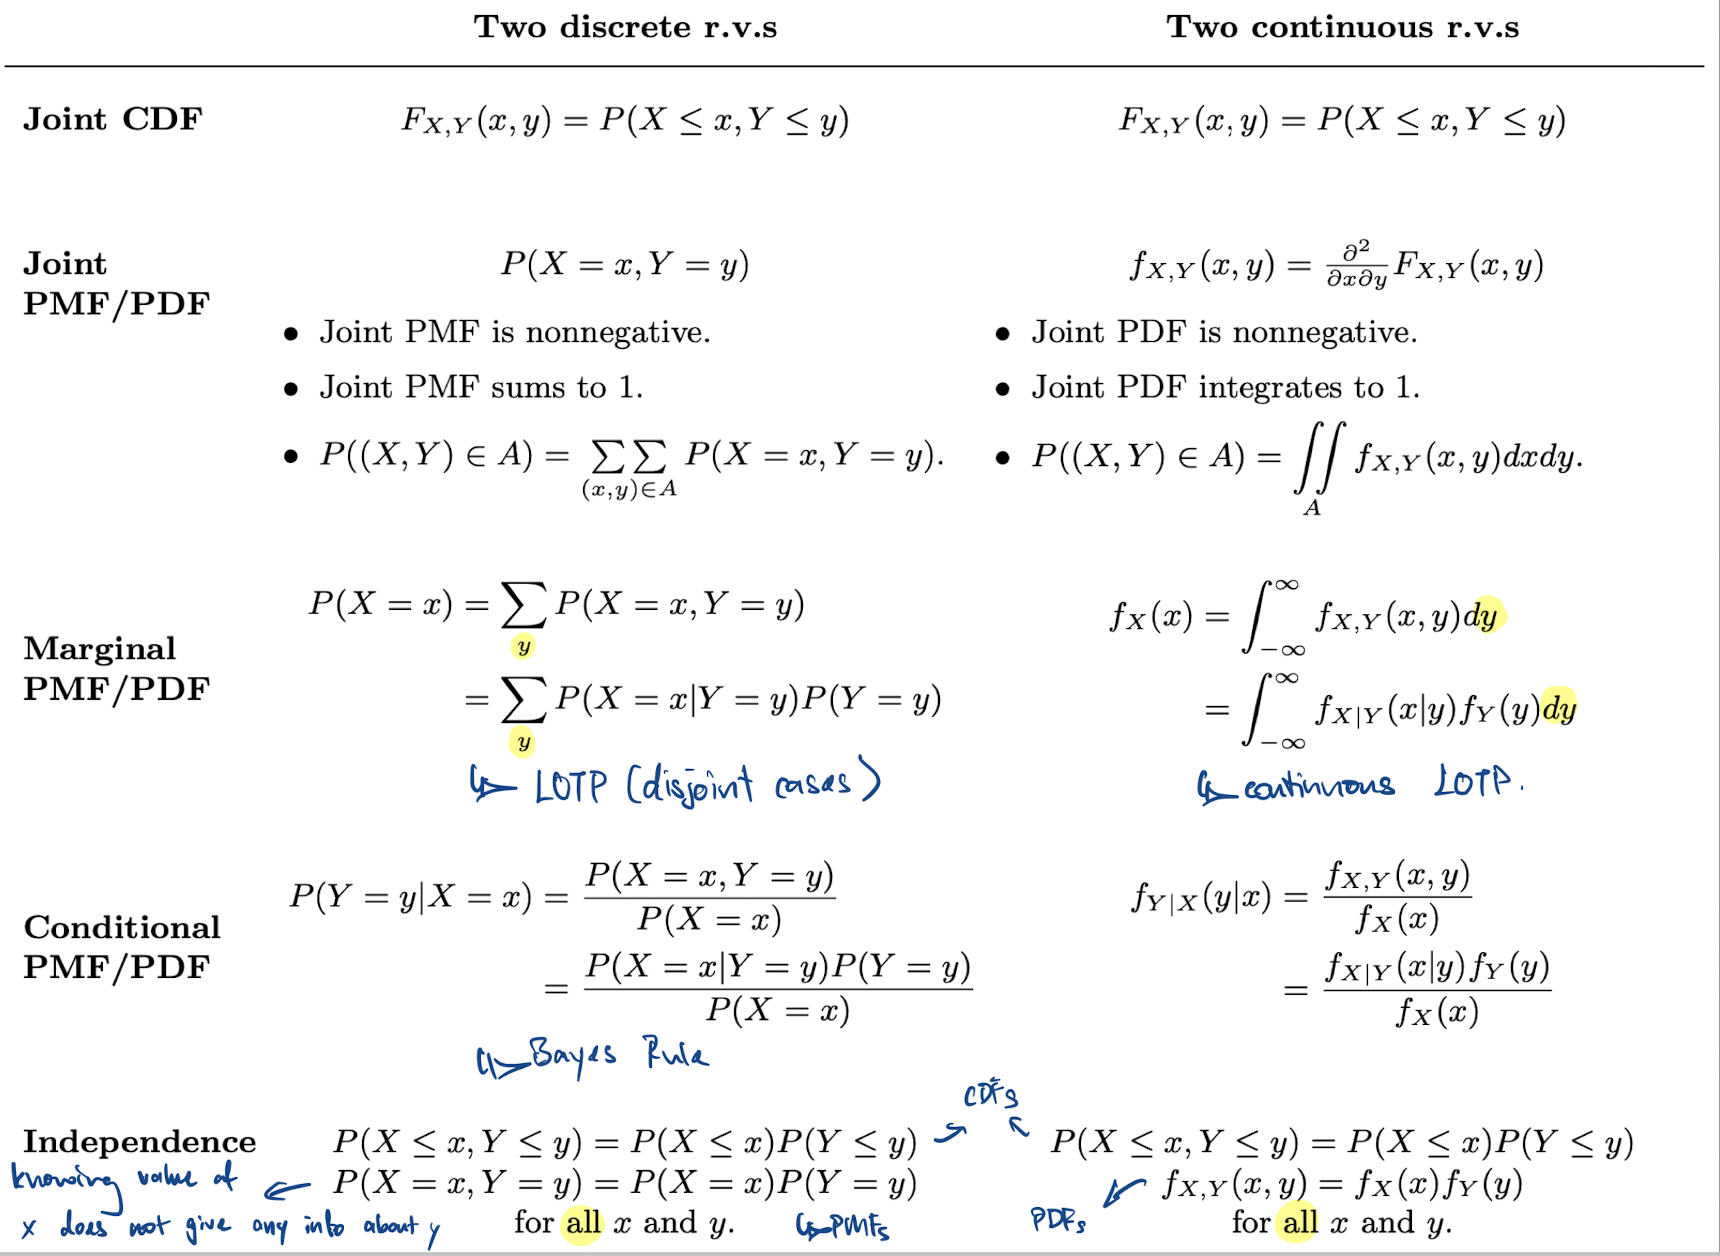
\includegraphics[scale=0.3]{./assets/jointDist}

		\highlight{Note}: Careful with limits of integration

		\textbf{Multinomial}:

		$n$ indiv, each in exactly 1 category, $p_i$ is prob of belonging to category i

		sum of $p_i$s = 1

		$X_i$ = \# of individuals in category i

		$\vec{X} \sim Mult_k(n, \vec{p})$, $X_j \sim Binom(n, p_j)$, dependent binomials

		\red{Lumping Property}: combine categories, still multinomial, probs add together\\

		\header{Moments}

		\textbf{Definition}: nth moment of X is $E(X^n)$

		1st moment: $E(X)$

		2nd moment: $E(X^2)$, Variance if $E(X) = 0$

		3rd moment: $E(X^3)$, related to skewness

		4th moment: $E(X^4)$, related to kurtosis

		\textbf{Moment Generating Function (MGF)}:

		MGF of $X$ is $M$, $M(t) = E(e^{tX})$

		1. Used to calc. Moments

		2. Determines a distribution uniquely

		3. Works well w sum of indep r.v, eg. X, Y indep

		\tab{} - Then $M_{X + Y}(t) = M_X(t)M_Y(t)$

		\textbf{Calculating Moments}

		$M(t) = E(e^{tX}) = E(\sum_{n = 0}^{\infty} \frac{(tX)^n}{n!}) = \sum \frac{E(X^n) t^n}{n!}$

		- nth moment is the coef. of $\frac{t^n}{n!}$ in taylor expansion of $M(t)$

		- $E(X^n)$ is the nth derivative of M evaluated at 0, $E(X^n) = M^{(n)}(0)$ 

		\red{Note}: $M(0) = 1$\\

		\header{Transformations and Convolutions}

		\textbf{Transformations}

		1. \textbf{Case 1: 1 dimension}

		$Y = g(X)$, where g is differentiable, strictly increasing, X is continuous

		\tab{} - Then, $f_Y(y) = f_X(x) |\frac{dx}{dy}|$, as a function of $Y$

		Proof: 
		
		1. $P(Y \leq y) = P(g(X) \leq y) = P(X \leq g^{-1}(y)) = F_X(x)$

		2. Differentiate both sides wrt to y, $f_Y(y) = f_X(x) |\frac{dx}{dy}|$

		2. \textbf{Case 2: n dimensions}

		$\vec{Y} = g(\vec{X}), \vec{X} = (X_1, X_2, \dots, X_n)$

		\tab{} - Then, $f_{\vec{Y}}(\vec{y}) = f_{\vec{X}}(\vec{x}) |\frac{\partial \vec{x}}{\partial \vec{y}}|$

		\tab{} - Absolute value of determinant of the jacobian matrix

		eg. $\frac{d(u, v)}{d(x, y)} = \left(
		\begin{matrix}
			\frac{du}{dx} & \frac{du}{dy} \\
			\frac{dv}{dx} & \frac{dv}{dy}
		\end{matrix}\right)$
		
		\textbf{Convolutions}: $X + Y = T$, X and Y indep

		1. Story, eg. with binomials

		2. MGF, but might not exist, hard to convert to PDF

		3. Convolution Sum or Integral

		1. \textbf{Discrete Case}: LOTP

		\centerline{$P(T = t) = \sum_{x} P(Y = t - x)P(X = x)$}

		2. \textbf{Continuous}: Convolution Integral

		\centerline{$f_T(t) = \int_{-\infty}{\infty} f_Y(t - x) f_X(x) dx$}
		
		\header{Order Statistics}

		PDF: $f_{X_{(j)}}(x) = n \binom{n-1}{j - 1} f(x)F(x)^{j-1}(1 - F(X))^{n - j}$\\

		\header{Conditional Expectation}

		\textbf{Conditional Expectation given an Event $A$}

		1. \textbf{Discrete}: $E(Y|A) = \sum_y yP(Y = y | A)$

		2. \textbf{Continuous}: $E(Y|A) = \int_{-\infty}^{\infty} y f(y|A) dy$

		\red{Note}: Linearity and other rules still hold

		\textbf{Law of Total Expection}: LOTE

		\centerline{$E(Y) = \sum_{j = 1}^n E(Y|B_j)P(B_j)$}

		\underline{Example}: Waiting for HH vs HT

		HT:

		1. wait for first H: FS(1/2)

		2. wait for first T after H: FS(1/2)

		$E(HT) = E(FS(1/2)) + E(FS(1/2)) = 2 + 2 = 4$

		HH: cannot ``build up progress'' like HT
		
		$E(HH) = E(HH | H_1)(1/2) + E(HH | T_1)(1/2)$

		$= (1/2(2) + 1/2(c + 2))(1/2) + (c + 1)(1/2)$, where c is E(HH)

		$=6$

		\textbf{Conditional Expectation given an r.v}: $g(X) = E(Y | X)$

		Properties:

		1. If indep, $E(Y|X) = E(Y)$

		2. $E(h(X)| X) = h(X)$ (completely dependent)

		3. $E(h(X)Y | X) = h(X)E(Y|X)$ (taking out whats known)

		4. Linearity

		\textbf{Adam's Law} (LOTE): $E(Y) = E(E(Y|X))$

		\textbf{Eve's Law} (total var): $Var(Y) = E(Var(Y|X)) + Var(E(Y|X))$\\

		\header{Inequalities}

		1. \textbf{Markov}: $P(|X| \geq a) \leq \frac{E|X|}{a}$ , $a > 0$

		\tab{} 1.1 Proof using indicator r.v.

		2. \textbf{Chebyshev}: $P(|X - \mu| \geq c \sigma) \leq \frac{1}{c^2}$

		3. \textbf{Cauchy-Schwarz}: $E|XY| \leq \sqrt{E(X^2)E(Y^2)}$

		\tab{} 3.1 find exact use 2D LOTUS
		
		\tab{} 3.2 find distribution use Jacobians transformation from $(x,y) \rightarrow (xy, x)$

		4. \textbf{Jensen}: If g is \underline{convex}: $E(g(X)) \geq g(E(X))$

		\tab{} 4.1 Convex: $g''(x) \geq 0$ or

		\tab{} 4.2 take any two points on function, line through them is above curve

		\tab{} 4.3 Variance $>$ 0 follows from this 

		\tab{} 4.4 if \underline{concave}: $E(h(X)) \leq h(EX)$\\

		\header{Limit theorems and Law of large numbers}

		\textbf{Sample Mean}:

		$X_1, X_2, \dots$ iid, mean $\mu$, variance $\sigma ^2$

		$\overline{X_n} = \frac{X_1 + \dots + X_n}{n}$, note sample mean is a r.v

		$E(\overline{X_n}) = \mu$, $Var = \sigma^2 / n$

		\textbf{Sample Variance}: 

		$s^2 = \frac{1}{n -1}\sum_{j = 1}^{n}(X_j - \overline{X_n})^2$

		$E(s^2) = \sigma^2$, $E(s) = E(\sqrt{s^2}) \leq \sqrt{Es^2} = \sigma$, by Jensen

		\textbf{Strong Law of Large Numbers}: $\overline{X_n} \rightarrow \mu$ with probability 1, as $n \rightarrow \infty$

		\textbf{Weak Law of Large Numbers}: 

		for any $\epsilon > 0$, 

		$P(|\overline{X_n} - \mu| \geq \epsilon) \rightarrow 0$ as $n \rightarrow \infty$, proof using Chebyshev

		\textbf{Central Limit Theorem}

		$T_n = \frac{\overline{X_n} - \mu}{\sigma / \sqrt{n}} \rightarrow N(0, 1)$, for large n

		$\overline{X_n} \sim N(\mu, \frac{\sigma^2}{n})$
		










	\end{multicols*}
\end{document}
